\documentclass[a4paper,12pt]{article}
\usepackage[utf8]{inputenc}
\usepackage[polish]{babel}
\usepackage[OT4]{polski}

\usepackage{graphicx}
\graphicspath{ {images/} }

\title{Metody odktywania wiedzy\\\Large{Dokumentacja końcowa}}
\author{Rafał Okuniewski, Maciej Zaborek}
\date{czerwiec 2017}

\begin{document}

\maketitle

\section{Wstęp}
\section{Wstępne przetwarzanie danych}
\section{Algorytmy selekcji atrybutów}
	\subsection{Stepwise Regression}
		Final Model:
count ~ onwaytowork + hours + weekdays + windspeed + humidity + 
    atemp + workingday + season
	\subsection{Regsubset analisys}
		\begin{figure}[h]
   			\centering
    		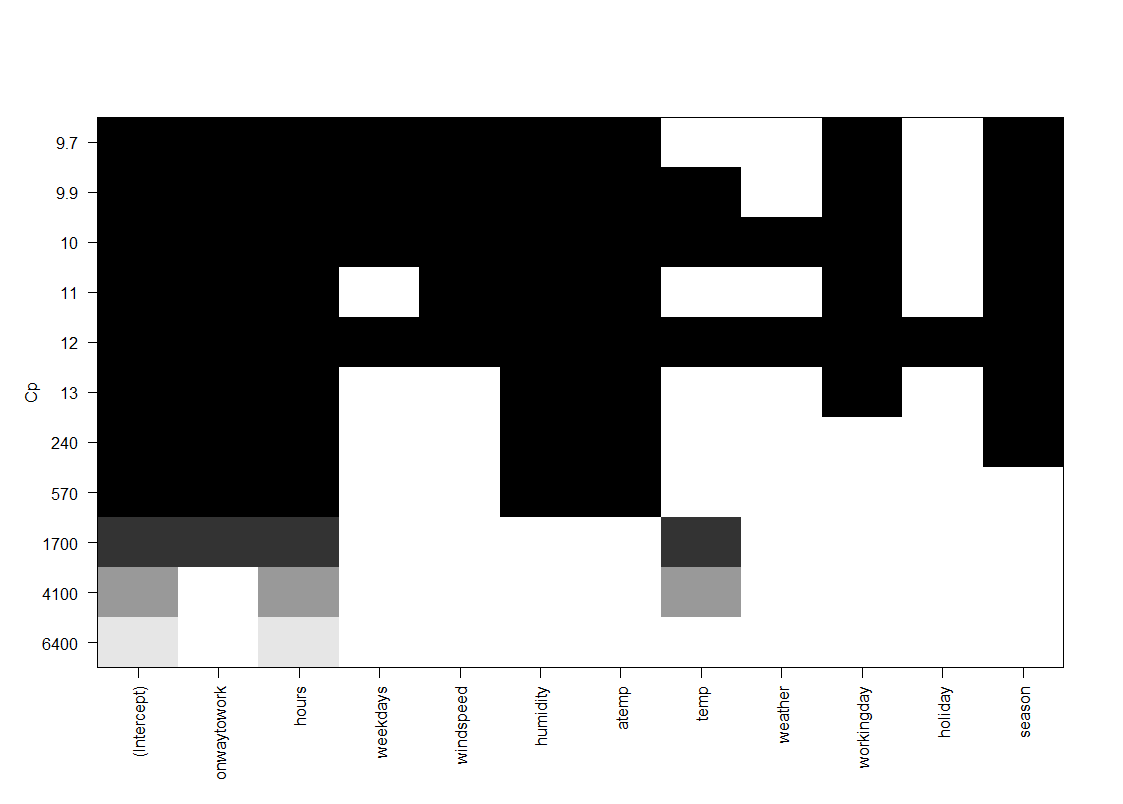
\includegraphics[width=\linewidth]{regsubsetanalysis}
		    \caption{Wyniki regsubset analisys}
    		\label{fig:my_label}
		\end{figure}
\section{Przetestowane algorytmy regresji}
    \subsection{Regresja liniowa}
    \begin{tabular}{|l|p{6cm}|r|r|}
\hline 
Liczba atrybutów & atrybuty & RMSLE & RMSE \\ 
\hline 
1 &  
hours 
 &  
1.328705
 &  
152.3693
 \\ 
\hline 
2 &  
hours + temp
 &  
1.236916
 &  
141.8473
 \\ 
\hline 
3 &  
onwaytowork + hours + temp
 &  
1.18398
 &  
129.6105
 \\ 
\hline 
4 &  
onwaytowork + hours + humidity + atemp
 &  
1.172317
 &  
123.351
 \\ 
\hline 
5 &  onwaytowork + hours + humidity + atemp + season 
 &  
1.171745
 &  
121.2109
 \\ 
\hline 
7 & onwaytowork + hours + windspeed + humidity + atemp + workingday + season &  
1.152467
 &  
119.855
 \\ 
\hline 
8 &  
onwaytowork + hours + weekdays + windspeed + humidity + atemp + workingday + season  
 &  
1.15163
 &  
119.8403
 \\ 
\hline 
\end{tabular} 
	\subsection{Regresja lokalna}
    \subsection{Robust regression z M-estymacją}
    \subsection{Drzewa regresji}

\section{Wnioski}

\end{document}
